% !TEX root = main.tex
\section{Second Order}
\label{sec:second}

At first order there is no gap (Proposition~\ref{prop:first-order}). This
section shows that there is one at the second-order type of a program with
two functional arguments, and describes the deterministic hull there.

\subsection{Sequential Programs and Kuhn's Theorem}
\label{sec:second-seq}

Let $X, Y, X', Y'$ be data types. The formula
$K = (X \multimap Y) \otimes (X' \multimap Y')$ is the \emph{core}. Its negation $T = K^{\perp}$ is the type of a program that receives two programs
$f : X \multimap Y$ and $g : X' \multimap Y'$, calls each once, and then
terminates or does not. Its web is $(X \times Y) \times (X' \times Y')$. A point $((a, b), (c, d))$ records that the program called $f$ on
$a$ and received $b$, and called $g$ on $c$ and received $d$. By
Definition~\ref{def:mall}(iii), $P(T)$ is the orthogonal of the products: it
is the set of $t$ with $\sum_{p, q} y_p\, t(p, q)\, z_q \le 1$ for all
$y \in P(X \multimap Y)$ and $z \in P(X' \multimap Y')$\leanref{p-second}. For
arguments $y$ and $z$, the sum $\sum_{p,q} y_p\, t(p,q)\, z_q$ is the
probability that $t$ terminates.

A \emph{randomized sequential program} of type $T$ calls one argument
first. If it calls $f$ first, it chooses the input $a$ with probability
$\mu(a)$, after the answer $b$ chooses the input $c$ to $g$ with
probability $\kappa(a, b, c)$, and after the answer $d$ terminates with
probability $\rho(a, b, c, d)$. Its value at $((a, b), (c, d))$ is
$\mu(a)\, \kappa(a, b, c)\, \rho(a, b, c, d)$ plus the analogous term for
the branch that calls $g$ first, with $\sum \mu \le 1$ over both branches,
$\sum_c \kappa(a, b, c) \le 1$, and $\rho \le 1$. It is
\emph{deterministic} if its values are in $\{0,1\}$. We prove the
following, whose part (ii) is an instance of Kuhn's
theorem~\cite{kuhn1953}.

\begin{theorem}[second order\leanref{sharp-td-iff}\leanref{sharp-mem-sequentialg}\leanref{recipe-eq-sequentialg}]
\label{thm:second-order}
Let $X$ and $X'$ be nonempty.
(i) A function with values in $\{0,1\}$ lies in $P(T)$ iff its support
lies in a set $\{((a, b), (c(b), d)) \mid b \in Y,\ d \in Y'\}$ for some
$a \in X$ and $c : Y \to X'$, or in a set
$\{((a(d), b), (c, d)) \mid b \in Y,\ d \in Y'\}$ for some $c \in X'$ and
$a : Y' \to X$. These are exactly the deterministic sequential programs.
(ii) The deterministic hull of $T$ is the set of randomized sequential programs.
\end{theorem}

\noindent
The two sets in (i) are the decision trees of a program that calls $f$
first and of one that calls $g$ first. Part (ii) has two directions. Every randomized
sequential program is a mixture of deterministic
ones\leanref{sequentialg-subset-mix}. Every mixture of randomized
sequential programs is a randomized sequential
program\leanref{mix-sequentialg}.

For nonempty $X$ and $X'$, we also prove that the deterministic hull of $T$ is the
set of denotations of a small language\leanref{proglang}\leanref{proglang-eq}. A program first
calls $f$ or $g$ on a fixed input, continues for each answer with a call
of the other function, and then terminates or not, with a finite
probabilistic choice $\mathsf{choose}(w_1 P_1, \dots, w_k P_k)$,
$\sum_i w_i \le 1$, at every stage. Every program denotes a randomized
sequential program\leanref{proglang-sound}. Every certain state of $T$
is a denotation\leanref{proglang-definable}. The language has no recursion. We do not relate it to probabilistic PCF
at this type, or the randomized sequential programs to the sequential
strategies of~\cite{castellan2018}.

\subsection{The Pentagon Gap}
\label{sec:second-pentagon}

The deterministic programs of type $X \multimap Y$ are its certain states,
the indicators of the graphs of partial functions. A pair $(f, g)$ of
deterministic programs \emph{produces} the point $((a, b), (c, d))$ if
$f(a) = b$ and $g(c) = d$. Two distinct points of the web of $T$ are
\emph{exclusive} if one pair of deterministic programs produces both, that
is, if they cohere in the core $K$. No certain state of $T$ gives the
value $1$ to two exclusive points, since its pairing with the product of
that pair of programs would be at least $2$. The \emph{exclusivity graph} of $T$ has the points of the web as
vertices and the exclusive pairs as edges. We show that $T$ has a gap.

\begin{figure}[t]
\centering
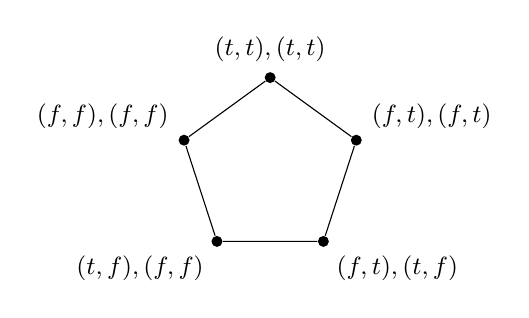
\begin{tikzpicture}[pt/.style={circle,fill,inner sep=1.4pt},
  every label/.style={font=\small}]
\node[pt,label={90:$(t,t),(t,t)$}]    (a) at (90:1.15) {};
\node[pt,label={18:$(f,t),(f,t)$}]    (b) at (18:1.15) {};
\node[pt,label={-54:$(f,t),(t,f)$}]   (c) at (-54:1.15) {};
\node[pt,label={-126:$(t,f),(f,f)$}]  (d) at (-126:1.15) {};
\node[pt,label={162:$(f,f),(f,f)$}]   (e) at (162:1.15) {};
\draw (a) -- (b) -- (c) -- (d) -- (e) -- (a);
\end{tikzpicture}
\caption{The five points of Theorem~\ref{thm:pentagon} over
$\mathrm{Bool}$, where $(a, b), (c, d)$ records $f(a) = b$ and
$g(c) = d$. Two points are joined when one pair of deterministic programs
produces both. The graph has no triangle, so the function with value
$\tfrac12$ on each point lies in $P(T)$. It has no three pairwise
non-adjacent points, so every randomized sequential program has total
weight at most $2$ on them.}
\label{fig:pentagon}
\end{figure}

\begin{theorem}[the pentagon\leanref{pente-not-mix}\leanref{pent-cycle}\leanref{pent-bounds}]
\label{thm:pentagon}
Let $X, Y, X', Y'$ have at least two elements each. There are five points
of the web of $T$ such that the function with value $\tfrac12$ on them and
$0$ elsewhere lies in $P(T)$ and not in the deterministic hull of $T$. For
$X = Y = X' = Y' = \mathrm{Bool}$, every randomized sequential program has
total weight at most $2$ on the five points, every element of $P(T)$ has
total weight at most $\tfrac52$ on them, and both bounds are attained.
\end{theorem}

\noindent
Over $\mathrm{Bool}$, write $(a, b)$ for the observation $f(a) = b$. The
five points are $((t,t),(t,t))$, $((t,f),(f,f))$, $((f,t),(t,f))$,
$((f,t),(f,t))$, and $((f,f),(f,f))$. They induce a cycle of length $5$ in the exclusivity graph
(Fig.~\ref{fig:pentagon}). The proof uses that this induced subgraph
has no triangle and no three pairwise non-adjacent vertices, which Lean checks by evaluation. It embeds the five points into larger types by
injections from $\mathrm{Bool}$. So no certain state gives the value $1$
to three of the five points. Hence $T$ has a gap: the function of the
theorem violates the counting law that bounds the total weight on the
five points by $2$.

The bounds $2$ and $\tfrac52$ are the independence number of the cycle
$C_5$ of length $5$, the largest number of pairwise non-adjacent vertices,
and its fractional relaxation. They are the noncontextual and the
exclusivity bounds of the KCBS scenario~\cite{cabello2014,klyachko2008}.

\subsection{Divergence and Total Programs}
\label{sec:second-total}

The function of Theorem~\ref{thm:pentagon} is partial: for some pairs of total functions it terminates with probability less
than $1$, for instance with probability $\tfrac12$ for $f$ the negation
and $g$ the identity on $\mathrm{Bool}$. At $T$ a
gap needs such partiality. Let $t \in P(T)$ terminate with probability $1$
on every pair of total functions. Constant arguments show that $t$ is a
conditional distribution of the inputs $(a, c)$ given the answers $(b, d)$. Termination with probability $1$ for all
total functions makes it a bipartite classical process without predefined causal
order~\cite{baumeler-wolf2016}. Every such process is a mixture of
processes in which one party acts first~\cite{baumeler-wolf2016}, and
these are randomized sequential programs. So $t$ lies in the deterministic hull of
$T$ by Theorem~\ref{thm:second-order}(ii). This argument is not
formalized. With three functional arguments,
we find a gap among the elements that terminate with probability $1$ on
every triple of total functions.

\begin{proposition}[a gap among total programs\leanref{gap-t3}]
\label{prop:t3}
Let $T_3 = ((\mathbf{2} \multimap \mathbf{2}) \otimes
(\mathbf{2} \multimap \mathbf{2}) \otimes
(\mathbf{2} \multimap \mathbf{2}))^{\perp}$. Some element of $P(T_3)$
terminates with probability $1$ on every triple of total functions and is
not in the deterministic hull of $T_3$.
\end{proposition}

\noindent
The element has value $1$ at one point of the web and $\tfrac12$ at
fourteen others. Since neither $\mathbf{2} \multimap \mathbf{2}$ nor its
tensor square has a gap, membership reduces to the $64$ triples of total
functions (proof of Theorem~\ref{thm:second-exact}). On each of them the
element has total weight exactly $1$. Five of its points with value
$\tfrac12$ form a cycle of length $5$ of exclusive pairs. So, as for
Theorem~\ref{thm:pentagon}, every mixture of certain states has total
weight at most $2$ on them, against $\tfrac52$. By the argument above,
the element is a tripartite classical process~\cite{baumeler-wolf2016}
that is not a mixture of deterministic ones. This identification is not
formalized.
